% !Mode\dots ``TeX:UTF-8''
% !TEX root = ../bare_jrnl.tex


\section{Introduction}
\label{sec:intro}


\IEEEPARstart{I}n 1960s, Nobel Prize laureates Jacob and Monod~\cite{Jacob1961Genetic} found that ``Any cell contains a number of regulatory genes that act as switches and can turn one another on and off. If genes can turn one another on and off, then you can have genetic circuits.'' Inspired by these Boolean-type actions in genetic circuits, Boolean networks (\BNs) were firstly proposed by Kauffman for modeling nonlinear and complex biological systems \cite{Kauffman1968Metabolic}. 

{\BNs} are a type of discrete-time dynamical systems which can be represented as directed graphs. A \BN\ $\BB$ starts at time $0$ from an {\em initial state} with given Boolean values of the nodes. At any time $t+1$ after it starts, the value $v(t+1)$ of a node $v$ of $\BB$ is determined by the values of the nodes at time $t$, i.e. $v_{i}(t),v_{j}(t),\ldots,v_k(t)$, which have edges to $v$ through a logic function. A large number of systems can be modelled as \BNs ~\cite{Kauffman1968Metabolic}, e.g. ~\cite{Akutsu2000Inferring, Shmulevich2002From, Faur2006Dynamical,Green2007The,Lou2010Multi}.

 %each node has only two values ``0" and ``1", and they can change in different time points.  For a node $n_i$, we use $n_i(t)$ to denote its value at time $t$.
%In general, $n_i(t+1)$ is determined by a logical function of $n_j(t),\ldots,n_p(t)$ if  there are  edges from $n_j,\ldots,n_p$ to $n_i$.  
%The logical operators used in  the logical functions include AND, OR, NO, XOR.  
%Some general descriptions of the \BNs\ and their applications to biological systems can be found in~\cite{Kauffman1968Metabolic}. There exists a large number of  systems, both natural and artificial, which are modelled as \BNs, e.g. ~\cite{Akutsu2000Inferring, Shmulevich2002From, Faur2006Dynamical,Green2007The,Lou2010Multi}.

Natural extensions of \BNs\ are Boolean control networks (\BCNs) with external regulations and perturbations~\cite{Ideker2001A}. \BCNs\ have been applied to  various real-life problems %. Cases of application can be found 
and typical examples from  structural and functional analysis of signaling and regulatory networks~\cite{Kaufman1999A, Klamt2006A}, 
abduction based drug target discovery~\cite{Biane2017Abduction}, 
and pursuing evasion problems in polygonal environments~\cite{Thunberg2011A}.
%

A \BCN\ has three distinguished finite sets of nodes $\{\mathsf{i}_1,\ldots\mathsf{i}_\ell\}$, $\{\mathsf{s}_1,\ldots\mathsf{s}_m\}$ and $\{\mathsf{o}_1,\ldots\mathsf{o}_n\}$ for some natural numbers $\ell$, $m$ and $n$, which are called the {\em input-nodes}, {\em state-nodes}  and {\em output-nodes}, respectively. At any time each node takes a Boolean value. The  timed behavior of $\BB$, i.e. the values of the state-nodes and output-nodes at any time points $t\ge0$ is determined by the initial values of the state nodes and the values of the input-nodes at each time point,  through the following {\em updating rules}.
\begin{itemize}
	\item The value $\mathsf{o}_i(t)$ of an output-node $\mathsf{o}_i$  is determined by the values of the state-nodes at time $t$, that is, there exist Boolean functions $h_i$ for $i=1,\ldots,n$ such that $\mathsf{o}_i(t)=\rho_i(\mathsf{s}_1(t),\ldots,\mathsf{s}_m(t))$; 
	\item the value $\mathsf{s}_j(t+1)$ of a state-node $\mathsf{s}_j$ at time point $t+1$ is determined by the values of the input-nodes and state-nodes at time point $t$, that is there are Boolean functions $f_j$ such that $\mathsf{s}_j(t+1)=\sigma_j(\mathsf{i}_1,\ldots,\mathsf{i}_\ell,\mathsf{s}_1(t),\ldots,\mathsf{s}_m(t))$ for $j=1,\ldots,m$.
\end{itemize}

 These functions are called the {\em updating rules} of $\BB$. We call a vector $\mathsf{i}=(\mathsf{i}_1,\ldots,\mathsf{i}_\ell )$ of Boolean valuations to the input-nodes an {\em input}, a vector $\mathsf{s}=(\mathsf{s}_1, \ldots, \mathsf{s}_m)$ of Boolean valuations to the state-nodes a {\em state}, and $\mathsf{o}=(\mathsf{o}_1,\ldots, \mathsf{o}_n)$ of Boolean valuations to the output-nodes an {\em output}. A {\em timed behavior} of $\BB$ at $t$ is given by the initial state $\mathsf{s}(0)$ and the output $\mathsf{o}(0)$ defined by the updating rules if $t=0$, and otherwise by the sequence $\mathsf{I}[t]=\mathsf{i}(0)\ldots\mathsf{i}(t-1)$ of inputs, the sequence $\mathsf{S}[t]=\mathsf{s}(1)\ldots\mathsf{s}(t)$ of states, and the sequence $\mathsf{O}[t]=\mathsf{o}(0)\ldots\mathsf{o}(t)$ of outputs such that
 
 \begin{itemize}
	\item if $t=0$ then $\mathsf{I}[t]$ is empty, and otherwise for $k=0,\ldots,t-1$, each $\mathsf{i}(k)$ is an input of $\BB$ at time point $k$;
	\item for $k=1,\ldots,t$, each $\mathsf{s}(k)$ is a state that is determined by $\mathsf{s}(k-1)$ and $\mathsf{i}(k-1)$ by the updating rules; and 
	\item for $k=0,\ldots,t$, each $\mathsf{o}(k)$ is an output that is determined by $\mathsf{s}(k)$ by the updating rules.
\end{itemize}

And we use $\mathsf{S}(t)$ to denote the set of possible valuations of $\mathsf{s}(t)$ of a \BCN\ $\BB$. With the sequence $\mathsf{I}[k]=\mathsf{i}(0)\ldots\mathsf{i}(k-1)$ of inputs and the sequence $\mathsf{O}[k]=\mathsf{o}(0)\ldots\mathsf{o}(k)$ of outputs of $\BB$. For $t=0,\ldots,k$,
 \begin{itemize}
	\item if $t=0$, the $\mathsf{S}(t)=\mathsf{S}(0)$ is determined by the output $\mathsf{o}(0)$ of $\BB$. That is for every $\mathsf{s}'(0)\in\mathsf{S}(0)$, the corresponding output $\mathsf{o}'(0)$ of $\mathsf{s}'(0)$ equals to the output $\mathsf{o}(0)$ of $\BB$.
	\item Otherwise, the $\mathsf{S}(t)$ is determined by $\mathsf{S}(t-1)$, $\mathsf{i}(t-1)$ and $\mathsf{o}(t)$. That is for every $\mathsf{s}'(t)\in\mathsf{S}(t)$, there is a $\mathsf{s}''(t-1)\in\mathsf{S}(t-1)$ such that the $\mathsf{s}''(t)$ which is determined by $\mathsf{s}''(t-1)$ and $\mathsf{i}(t-1)$  equals to $\mathsf{s}'(t)$  and the corresponding output $\mathsf{o}'(t)$ of $\mathsf{s}'(t)$ equals to the output $\mathsf{o}(t)$ of $\BB$.
\end{itemize}


 In general when constructing a \BCN\ model of dynamic systems or working with a system built from a \BCN, \BCN\ is a blackbox and the state of the system is hidden. One can only control the inputs and observe output, without knowing or being able to observe the changes of the states frome time to time. As being pointed in ~\cite{Akutsu2007Control}, a major goal to study a kind of systems using \BCNs\ is to develop a control theory to deal with the following three fundamental issues \cite{cheng2009controllability, Zhao2010Input, Cheng2011Identification, Cheng2011Analysis} and \cite{Fornasini2013Observability}.
  
% And a user can only control the  values of the input-nodes and observe those of the output-nodes, without being able to observe the values of the state-nodes change from time to time. We use an {\em input vector} $\mathsf{i}(t)=(\mathsf{i}_1(t),\ldots,\mathsf{i}_\ell (t))$, a {\em state vector} $\mathsf{s}(t)=(\mathsf{s}_1(t), \ldots, \mathsf{s}_m(t))$ and an {\em output  vector} $\mathsf{o}(t)=(\mathsf{o}_1(t),\ldots, \mathsf{o}_n(t))$  to represent an assignment of Boolean values to the  input-nodes, state-nodes and  output-nodes at $t$, respectively.  We call them an {\em input}, a {\em state} and an {\em output} of the \BCN\ at time time $t$. As  illustrated by Fig.~\ref{fig:10},  the state $\mathsf{s}(t+1)$ at time $t+1$ is determined by the input $\mathsf{i}(t)$ and state $\mathsf{s}(t)$ at $t$  and the output $\mathsf{o}(t)$  is determined by the state  $\mathsf{s}(t)$.  We call a state $\mathsf{s}(0)$ at time $0$ an {\em initial state}. Thus, for any $k>0$, the state sequence  $\mathsf{S}[k]=\mathsf{s}(1)\ldots\mathsf{s}(k)$ and the output sequence $\mathsf{O}[k]=\mathsf{o}(0)\ldots\mathsf{o}(k)$ are  determined by an  input sequence $\mathsf{I}[k]=\mathsf{i}(0)\ldots\mathsf{i}(k-1)$ and initial state $\mathsf{s}(0)$. 

%With the need of capturing the ability to guide a \BCN\ to a desired state through a suitable choice of inputs, the {\em controllability} was proposed. And with the need of capturing the ability to determine a \BCN's initial state by its inputs and outputs, the {\em observability}  was proposed. Controllability and observability motivate active research on their related {\em control-theoretic problems}, e.g.  \cite{cheng2009controllability, Zhao2010Input, Cheng2011Identification, Cheng2011Analysis} and \cite{Fornasini2013Observability}, which we summarize below.


%Thus,  we cannot observe how the values of the state-nodes change from time to time. Therefore, it is important to find a way to determine the initial values of the state-nodes at $0$ after observing a sequence of values of  input-nodes and their corresponding  values of the output-nodes. This is in general known as the {\em observability} of a \BCN.



% is one of the two basic  properties related to  the control-theoretic problems of \BCNs. The other is known as {\em controllability}.  Since then, research on  controllability and observability of \BNs\ and \BCNs\ has drawn a great attention, e.g. \cite{cheng2009controllability, Zhao2010Input, Cheng2011Identification, Cheng2011Analysis} and \cite{Fornasini2013Observability}.

%The concept of observability was first proposed in~\cite{cheng2009controllability}. After that, four types of observability have been investigated in the literature which we will discuss below.
%There are three kinds of nodes in \BCNs:  {\em input-nodes}, {\em state-nodes}  and {\em output-nodes}. At any  time each node takes a Boolean value.  The value of an output-node at time point $t$ (where $t\geq 0$)  depends on the values of state-nodes at time $t$, but the value of a  state-node at time point $t+1$  is determined by a  Boolean function of the values of the input-nodes and state-nodes at time point $t$.  These relations between nodes are presented by the updating rules of \BCN.  However,  we can only control the  values of the input-nodes and observe those of the output-nodes. We cannot observe how the values of the state-nodes change from time to time.
%Therefore, it is important to find a way to determine the initial values of the state-nodes at $0$ after observing a sequence of values of  input-nodes and their corresponding  values of the output-nodes. This is in general known as the {\em observability} of a \BCN.

%The identification of \BCNs\ was proposed in~\cite{Cheng2011Identification}. It is about how to determine the updating rules of a \BCN\ from the values of  input-nodes  and output-nodes at a sequence of time points $0,\ldots, k$. And it is an important topic, for example, we may be interested in the updating rules of a \BCN\ which presents a real celluar network. 

%Observability is one of the two basic  properties related to  the control-theoretic problems of \BCNs. The other is known as {\em controllability}. The work in ~\cite{Akutsu2007Control} shows that the problem of determining the controllability of \BCNs\ is {NP}-hard. Moreover, it  points out that ``One of the major goals of systems biology is to develop a control theory for complex biological systems.''  Since then, research on  controllability and observability of \BNs\ and \BCNs\ has drawn a great attention, e.g. \cite{cheng2009controllability, Zhao2010Input, Cheng2011Identification, Cheng2011Analysis} and \cite{Fornasini2013Observability}. %There, it is further noted that the controllability and observability are the basic control-theoretic problems of \BCNs. % Among these studies, \emph{semi-tensor product} (\STP) is one of useful tools to deal with  

 %The concept of observability was first proposed in~\cite{cheng2009controllability}. It is mainly about how  to determine  the values of the  state-nodes  of a \BCN\  at time $0$ from the values of  input-nodes  and output-nodes at a sequence of time points $0,\ldots, k$. After that, four types of observability have been investigated in the literature, together with their corresponding determining algorithms, which we will discuss below.

\begin{figure}[!t]
      \centering
      \framebox{\parbox{3in}{
		\centerline{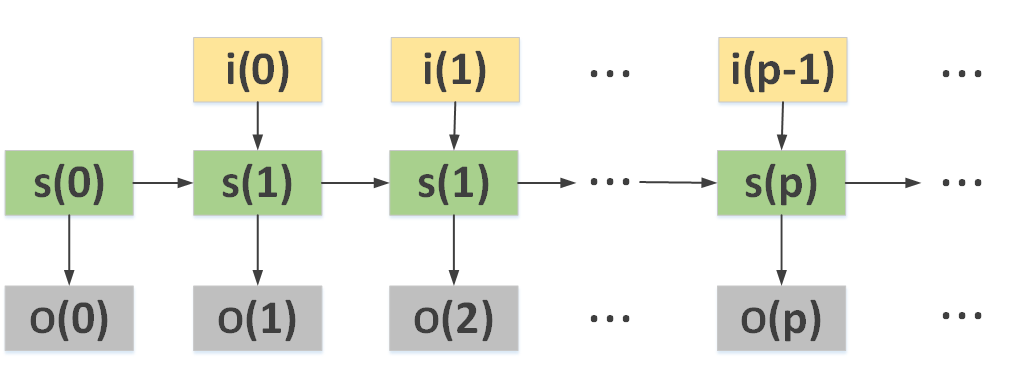
\includegraphics[scale=0.17]{figures/Fig10.png}}
	}}
      
      \caption{The relationship of inputs, states and outputs.}
      \label{fig:10}
  \end{figure}

%Given a \BCN\ with $\ell$ input-nodes $(\mathsf{i}_1,\ldots, \mathsf{i}_\ell)$, $m$ state-nodes $(\mathsf{s}_1,\ldots, \mathsf{s}_m)$ and $n$ output notes  $(\mathsf{o}_1,\ldots, \mathsf{o}_n)$,  

%The notions of controllability and observability of \BCNs\ can thus be described as follows.
{\em The identifiability problem}: This is about it is possible and how to find the updating rules of a \BCN\ $\BB$ by providing sequence of inputs (and observing the corresponding sequence of outputs), especially when the mechanism for setting $\BB$ with different initial states is not available~ \cite{Cheng2011Identification}.

{\em The controllability problem}: %Controllability of \BCNs\ is investigated in ~\cite{Akutsu2007Control}. 
This about if it is possible and how for a given initial state to find a sequence of inputs by the updating rules, such that the behavior of a \BCN\ $\BB$ corresponding to the sequence of inputs will reach a desired state~\cite{Akutsu2007Control}.
%A \BCN\ $\BB$ is controllable if given any initial state $\mathsf{s}$ and destination state $\mathsf{s}'$, there exists an input sequence $\mathsf{I}[k]=\mathsf{i}(0)\ldots\mathsf{i}(k-1)$ for some $k>0$ such that $\mathsf{S}[k]=\mathsf{s}(1)\ldots\mathsf{s}(k)$ is the corresponding sequence of state updates from the initial state $\mathsf{s}$ to the destination state $\mathsf{s}'$ produced by $\mathsf{I}[k]$, i.e. $\mathsf{s}(0)=s$ and $\mathsf{s}(k)=\mathsf{s}'$. It is shown in ~\cite{Akutsu2007Control} that the problem of determining the controllability of \BCNs\ is {NP}-hard. There, it further states that controllability of \BCNs\ is important to the development of a control theory for complex biological systems.
%That is for a given  \BCN\  $\BB$,  $\mathsf{o}(0)\mathsf{o}(1)\ldots\mathsf{o}(k)$ is decide by $\mathsf{s}(0)$ and the sequence $\mathsf{i}(0)\mathsf{i}(1)\ldots\mathsf{i}(k-1)$. 
%

{\em The observability problem}: This is about it is possible and how to determine the intial state of a \BCN\ $\BB$ by providing sequences of inputs and observing the corresponding output sequences  based on the updating rules~\cite{cheng2009controllability}. There are four types of observability have been investigated in the literature, which are described below.
%The concept of observability is proposed in 2009 ~\cite{cheng2009controllability}. It is about how to determine the initial state $\mathsf{s}(0)$ of a \BCN\ from the sequence of values of the input-nodes and its corresponding sequence of values of the output-nodes. Since then, four types of observability have been investigated in the literature, which are described below.

%The identifiability of \BCNs\ can thus be described as follows. 

%{\em Identifiability}:A \BCN\ $\BB$ is identifiable if its updating rules can be determined via its input-output data $\mathsf{i}(0)\ldots\mathsf{i}(k-1)$ and $\mathsf{o}(0)\ldots\mathsf{o}(k)$. Precisely speaking, there is an input sequence $\mathsf{I}=\mathsf{i}(0)\ldots\mathsf{i}(k-1)$ for some $k>0$ which produces output sequence $\mathsf{O}=\mathsf{o}(0)\ldots\mathsf{o}(k)$, such that the updating rules of $\BB$ can be determined via $\mathsf{I}$ and $\mathsf{O}$ \cite{Cheng2011Identification}.
\begin{enumerate}
\item The  {\bf type-I}  observability was proposed in 2009 ~\cite{cheng2009controllability}. It states that a \BCN\ $\BB$ is observable if for any initial state   $\mathsf{s}(0)$ there exists an input sequence  $\mathsf{I}[k]=\mathsf{i}(0)\ldots\mathsf{i}(k-1)$ which can  distinguish $\mathsf{s}(0)$ from any other initial state $\mathsf{s}'(0)$. That is,  given any initial state $\mathsf{s}(0)$, there is an input sequence $\mathsf{I}[k]=\mathsf{i}(0)\ldots\mathsf{i}(k-1)$ for some $k>0$ such that  for any  $\mathsf{s}'(0)$ which is different from $\mathsf{s}(0)$, the output sequence  $\mathsf{O}[k]=\mathsf{o}(0)\ldots\mathsf{o}(k)$ produced by  $\mathsf{s}(0)$ and $\mathsf{I}[k]$ is different the output sequence  $\mathsf{O}'[k]=\mathsf{o}'(0)\ldots \mathsf{o}'(k)$ produced by  $\mathsf{s}'(0)$ and $\mathsf{I}[k]$.

Assume a \BCN\ $\BB$  with {\bf type-I}  observability, and we determine the set $\mathsf{S}(0)$ of possible valuations of initial state $\mathsf{s}(0)$ by the output $\mathsf{o}(0)$. 
%Then, for each initial state $\mathsf{s}'(0)\in \mathsf{S}(0)$, there is an input sequence $\mathsf{I}'[k]=\mathsf{i}'(0)\ldots\mathsf{i}'(k-1)$ for which the corresoning output sequnece $\mathsf{O}'[k]=\mathsf{o}'(0)\ldots\mathsf{o}'(k)$ of $\mathsf{s}'(0)$ is different from the output sequence $\mathsf{O}''[k]=\mathsf{o}''(0)\ldots\mathsf{o}''(k)$ for any different initial state $\mathsf{s}''(0)\in \mathsf{S}(0)$ with the same inpout sequnece. 
Thus, we have foloiwng procedure to determe the initial state $\mathsf{s}(0)$.
\begin{description}
	\item[Step 1] Set variable $\mathsf{S}$ be set to $\mathsf{S}(0)$.
	\item[Step 2] Choose a initial state $\mathsf{s}'(0)$ from $\mathsf{S}$, input to the \BCN\ $\BB$ with the input sequence $\mathsf{I}'[k]$, which distinguish $\mathsf{s}'(0)$ from other initial states, and run $\BB$ to generate the output sequence $\mathsf{O}[k]=\mathsf{o}(0)\ldots\mathsf{o}(k)$.
	\item[Step 3] If the ouput sequence $\mathsf{O}[k]=\mathsf{o}(0)\ldots\mathsf{o}(k)$ is the same as the output sequence $\mathsf{O}'[k]=\mathsf{o}'(0)\ldots\mathsf{o}'(k)$ for $\mathsf{s}'(0)$, then return $\mathsf{s}'(0)$ as the initial state of $\BB$. Otherwise, set $\mathsf{S}=\mathsf{S}-\{\mathsf{s}'(0)\}$ by removing $\mathsf{s}'(0)$ from the $\mathsf{S}$, and go to Step 2.
	
\end{description}
\item The  {\bf type-II} observability was proposed in 2010 \cite{Zhao2010Input}. It states that a \BCN\ $\BB$ is observable if for every two different initial states $\mathsf{s}(0)$ and $\mathsf{s}'(0)$, there exists an input sequence $\mathsf{I}[k]=\mathsf{i}(0)\ldots\mathsf{i}(k-1)$ that can distinguish $\mathsf{s}(0)$ and $\mathsf{s}'(0)$. More precisely speaking,  for any pair of different initial  $\mathsf{s}(0)$ and $\mathsf{s}'(0)$, there exists an input sequence  $\mathsf{I}[k]=\mathsf{i}(0)\ldots\mathsf{i}(k-1)$ for some $k>0$ such that the output sequences $\mathsf{O}[k]=\mathsf{o}(0)\ldots\mathsf{o}(k)$ and  $\mathsf{O}'[k]=\mathsf{o}'(0)\ldots\mathsf{o}'(k)$ corresponding to  the different initial states  $\mathsf{s}(0)$ and $\mathsf{s}'(0)$, respectively, are different.
	
	Assume a \BCN\ $\BB$  with {\bf type-II}  observability, and we determine the set $\mathsf{S}(0)$ of possible valuations of initial state $\mathsf{s}(0)$ by the output $\mathsf{o}(0)$. 
	%Then, for every two different initial states $\mathsf{s}'(0), \mathsf{s}''(0)\in \mathsf{S}(0)$, there is a correspdining input sequence $\mathsf{I}'[k]=\mathsf{i}'(0)\ldots\mathsf{i}'(k-1)$ for which the corresoning output sequnece $\mathsf{O}'[k]=\mathsf{o}'(0)\ldots\mathsf{o}'(k)$ is different from the output sequence $\mathsf{O}''[k]=\mathsf{o}''(0)\ldots\mathsf{o}''(k)$ for the initial state $\mathsf{s}''(0)$ with the same inpout sequnece. 
	Thus, we have foloiwng procedure to determe its initial state $\mathsf{s}(0)$.
\begin{description}
	\item[Step 1]  Set variable $\mathsf{S}$ be set to $\mathsf{S}(0)$.
	\item[Step 2] Choose two initial states $\mathsf{s}'(0)$ and $\mathsf{s}''(0)$ from $\mathsf{S}$, input to the \BCN\ $\BB$ with the input sequence $\mathsf{I}'[k]$, which distinguish $\mathsf{s}'(0)$ and $\mathsf{s}''(0)$, and run $\BB$ to generate the output sequence $\mathsf{O}[k]=\mathsf{o}(0)\ldots\mathsf{o}(k)$.
	\item[Step 3] With the input sequence $\mathsf{I}'[k]$ and output sequence $\mathsf{O}[k]$, we can further determine $\mathsf{S}(0)$. That is, for every $\mathsf{s}^*(0)\in\mathsf{S}(0)$, the output sequence $\mathsf{O}^*[k]=\mathsf{o}^*(0)\ldots\mathsf{o}^*(k)$ produced by $\mathsf{s}^*(0)$ and $\mathsf{I}'[k]$ equals to $\mathsf{O}[k]$.
	\item[Step 4] Set $\mathsf{S}=\mathsf{S}\cap\mathsf{S}(0)$ by the intersection of $\mathsf{S}(0)$ and $\mathsf{S}$. If the cardinal number $|\mathsf{S}|=1$, then return the $\mathsf{s}'(0)$ belonging to $\mathsf{S}$ as the initial state of $\BB$. Otherwise, go to Step 2.
\end{description}
	
\item The  {\bf type-III} observability was proposed in 2011 \cite{Cheng2011Identification}.  It states that a \BCN\ $\BB$ is observable if there is an input sequence $\mathsf{I}[k]=\mathsf{i}(0)\ldots\mathsf{i}(k-1)$ that distinguishes all different initial states. This means that in $\BB$, there exists an input sequence  $\mathsf{I}[k]=\mathsf{i}(0)\ldots\mathsf{i}(k-1)$ for some $k>0$ such that for any two different initial states $\mathsf{s}(0)$ and $\mathsf{s}'(0)$, the output sequence $\mathsf{O}[k]=\mathsf{o}(0)\ldots\mathsf{o}(k)$  corresponding to  $\mathsf{s}(0)$  is different from the output sequence  $\mathsf{O}'[k]=\mathsf{o}'(0)\ldots\mathsf{o}'(k)$ corresponding to $\mathsf{s}'(0)$.
%\JP{Please don't change notations. Stick to $s(0)$ and $s'(0)$. $\mathsf{s}^{x}(0)$ and $\mathsf{s}^{y}(0)$ are somehow strange.}

Assume a \BCN\ $\BB$  with {\bf type-III}  observability, then there is an input sequence $\mathsf{I}[k]=\mathsf{i}(0)\ldots\mathsf{i}(k-1)$ for some $k>0$ such that for all ${2^m}$ different initial states $\mathsf{s}^1(0),\ldots, \mathsf{s}^{2^m}(0)$ of $\BB$ ($m$ is the number of state-nodes), their corresponding output sequences $\mathsf{O}^1[k]=\mathsf{o}^1(0)\ldots\mathsf{o}^1(k),\ldots, \mathsf{O}^{2^m}[k]=\mathsf{o}^{2^m}(0)\ldots\mathsf{o}^{2^m}(k)$ are different. Thus, we have followng procedure to determe $\mathsf{s}(0)$.

 \begin{description}
	\item[Step 1]  Input to the \BCN\ $\BB$ with the input sequence $\mathsf{I}[k]$ which distinguishes all different initial states $\mathsf{s}^1(0),\ldots, \mathsf{s}^{2^m}(0)$, and run $\BB$ to generate the output sequence $\mathsf{O}[k]=\mathsf{o}(0)\ldots\mathsf{o}(k)$.
	\item[Step 2]  If the output sequence $\mathsf{O}'[k]$ produced by $\mathsf{s}'(0)$ and $\mathsf{I}[k]$ is the same as $\mathsf{O}[k]$, then return $\mathsf{s}'(0)$ as the initial state of $\BB$.
\end{description}
	
\item  The  {\bf type-IV}  observability was  proposed in 2013 \cite{Fornasini2013Observability}. It states that a \BCN\ $\BB$ is observable if every sufficient long $\mathsf{I}[k]=\mathsf{i}(0)\ldots\mathsf{i}(k-1)$ genertaes different output sequences  from different initial states. Precisely speaking, there is a big enough number $M$, for every  input sequence $\mathsf{I}[k]$ which is not shorter than $M$, the output sequences $\mathsf{O}[k]=\mathsf{o}(0) \ldots\mathsf{o}(k)$ and  $\mathsf{O}'[k]=\mathsf{o}'(0)\ldots\mathsf{o}'(k)$ produced by the input sequence $\mathsf{I}[k]$ from every two different initial states $\mathsf{s}(0)$ and $\mathsf{s}'(0)$, respectively, are different.

Assume a \BCN\ $\BB$  with {\bf type-IV}  observability. Then, there is a big enough number $M$, for every  input sequence $\mathsf{I}[k]=\mathsf{i}(0)\ldots \mathsf{i}(k-1)$ which is not shorter than $M$,   for all ${2^m}$ different initial states $\mathsf{s}^1(0),\ldots, \mathsf{s}^{2^m}(0)$ of $\BB$, their corresponding output sequences $\mathsf{O}^1[k]=\mathsf{o}^1(0)\ldots\mathsf{o}^1(k),\ldots, \mathsf{O}^{2^m}[k]=\mathsf{o}^{2^m}(0)\ldots\mathsf{o}^{2^m}(k)$ are different. Thus, we have followng procedure to determe $\mathsf{s}(0)$.
 \begin{description}
	\item[Step 1]  Input to the \BCN\ $\BB$ with an arbitrary input sequence $\mathsf{I}[k]=\mathsf{i}'(0)\ldots \mathsf{i}'(k-1)$ which is not shorter than $M$, and run $\BB$ to generate the output sequence $\mathsf{O}[k]=\mathsf{o}(0)\ldots\mathsf{o}(k)$.
	\item[Step 2]  If the output sequence $\mathsf{O}'[k]$ produced by $\mathsf{s}'(0)$ and $\mathsf{I}[k]$ is the same as $\mathsf{O}[k]$, then return $\mathsf{s}'(0)$ as the initial state of $\BB$.
\end{description}
\end{enumerate}
%We will give the formal definitions of these four types of observability and discussion their relations in Section~\ref{sec:pre}.
 %We will give the formal definition of identifiability in Section~\ref{sec:pre}. And in this paper \cite{Cheng2011Identification}, the author claims that a \BCN\ is identifiable iff it is controllable and observable. The controllability and observability are described as follows. 
 %\JP{So far, I don't see a clear difference among the first three types from the above description.}

Each of these types of observability is used to solve a kind of problems of \BCNs. The {\bf type-I}  observability is proposed to determine the initial state $\mathsf{s}(0)$ of \BCN\ whose initial state $\mathsf{s}(0)$ can be reset. %, or alternatively having a number of copies of the original \BCN, all in the same initial state. 
And with further research, people proposed the {\bf type-II} observability to capture the ability to determine the initial state $\mathsf{s}(0)$ of \BCN\ whose initial state $\mathsf{s}(0)$ can be reset, i.e. the $\mathsf{s}(0)$ can be determined iff the \BCN\ satisfies the {\bf type-II} observability. The {\bf type-III} observability is proposed to research the {\em identification problem} of \BCN\ because it can be used to determine the initial state $\mathsf{s}(0)$ of \BCN\ whose initial state $\mathsf{s}(0)$ can not be reset. The {\bf type-IV} observability was proposed in~\cite{Fornasini2013Observability}, it captures the ability to determine the initial state of a \BCN\ whose initial state $\mathsf{s}(0)$ can not be reset by  inputing an arbitrary sufficient long input sequence and observing the outputs of \BCN. In~\cite{Fornasini2013Observability}, the reconstructibility of \BCNs\ was investigated too.
It states that a \BCN\ $\BB$ is reconstructible if there is a big enough number $M$, for every  input sequence $\mathsf{I}[k]=\mathsf{i}(0)\ldots \mathsf{i}(k-1)$ which is not shorter than $M$, we can determine the $\mathsf{s}(k)$ of $\BB$ by the $\mathsf{I}[k]$ and the output sequence  $\mathsf{O}[k]=\mathsf{o}(0)\ldots\mathsf{o}(k)$ of $\BB$. And the {\bf type-IV} observability implies the reconstructibility. %And we found the {\bf type-III} observability not good enough for the the identification problem.
%Loosely speaking, different types of observability were proposed for different applications. For instance, the {\bf type-IV} observability was proposed to research the reconstructibility of \BCN, and the {\bf type-III} observability was proposed to research the {\em identification problem} of \BCN. And we found the {\bf type-III} observability not good enough for the the identification problem.

In this paper, we study the weakness of {\bf type-III} observability for identification problem.

{\em The identification problem}: A \BCN\ $\BB$ is identifiable if the updating rules can be determined by an input sequence $\mathsf{I}[k]=\mathsf{i}(0)\ldots\mathsf{i}(k-1)$ and the corresponding output sequence $\mathsf{O}[k]=\mathsf{o}(0)\ldots\mathsf{o}(k)$ for some $k>0$~ \cite{Cheng2011Identification}. The identification problem of \BCNs\ was proposed in~\cite{Cheng2011Identification} to determine the updating rules of a \BCN\ by repeatedly feeding inputs to the input-nodes and observing the corresponding values generated by the output-nodes. 
There further states that a \BCN\ $\BB$ is identifiable iff it satisfies two conditions. The first one is the controllability, and the second one is the initial state $\mathsf{s}(0)$ of $\BB$ can be determined even if the $\mathsf{s}(0)$ can not be reset. %We will give the proof of this proposition in {\bf Appendix~A~Proof}. %, we have that we need to determine the initial state of a \BCN\ to identify its updating rules.
%We will give its formal definition in Section~\ref{sec:pre}. 

The authors of~\cite{Cheng2011Identification} claim that a \BCN\ is identifiable iff it satisfies controllability and the {\bf type-III} observability. But we found that the {\bf type-III} observability does not capture the ability to determine the initial state $\mathsf{s}(0)$ of \BCN\ whose initial state $\mathsf{s}(0)$ can not be reset. We can also determine the initial state $\mathsf{s}(0)$ of a \BCN\ $\BB$ whose $\mathsf{s}(0)$ can not be reset, if it satisfies the {\bf type-IV} observability. But the {\bf type-IV} observability implies the {\bf type-III} observability, so the {\bf type-IV} observability does not capture the ability to determine the initial state $\mathsf{s}(0)$ of \BCN\ whose initial state $\mathsf{s}(0)$ can not be reset either. Thus we propose a new type of observability to research identification problem. 

Firstly, for the set $\mathsf{S}(t)$ of possible valuations of $\mathsf{s}(t)$ of a \BCN\ $\BB$, 
 \begin{itemize}
	\item we can determine the $\mathsf{s}(t)$ of $\BB$ at time point $t$ for every $\mathsf{s}(t)\in \mathsf{S}(t)$, iff the cardinal $|\mathsf{S}(t)|=1$.
	\item And  we can determine the $\mathsf{s}(t)$ of $\BB$ at time point $t+k$ for some $k>0$ for every $\mathsf{s}(t)\in \mathsf{S}(t)$, iff there is an input $\mathsf{i}(t)$ 
	\begin{itemize}
	\item which would not make every two distinct states $\mathsf{s}'(t)$, $\mathsf{s}''(t)$$\in$ $\mathsf{S}(t)$ become the same state after affected by $\mathsf{i}(t)$,
	 \item and for every possible output $\mathsf{o}(t+1)$ we may observe, the $\mathsf{S}(t+1)$ determined by $\mathsf{S}(t)$, $\mathsf{i}(t)$ and $\mathsf{o}(t+1)$ satisfies that we can determine the $\mathsf{s}(t+1)$ of $\BB$ at or before time point $((t+1)+(k-1))$ for every $\mathsf{s}(t+1)\in \mathsf{S}(t+1)$.
	 \end{itemize}
\end{itemize}
%Firstly, we propose a new algorithm to determine the initial state $\mathsf{s}(0)$ of a \BCN\ $\BB$ as follows.



%{\em Observability}:A \BCN\ $\BB$ is observable if there is an input sequence $\mathsf{i}(0)\ldots\mathsf{i}(k-1)$ that distinguishes every pair of different initial states. This means that in $\BB$, there exists an input sequence  $\mathsf{i}(0)\ldots\mathsf{i}(k-1)$ for some $k>0$ such that for any two different initial states $\mathsf{s}(0)$ and $\mathsf{s}'(0)$, the output sequence $\mathsf{o}(0)\ldots \mathsf{o}(k)$  corresponding to  $\mathsf{s}(0)$  is different from the output sequence  $\mathsf{o}'(0)\ldots\mathsf{o}'(k)$ corresponding to $\mathsf{s}'(0)$.

 %We will give its formal definition in Section~\ref{sec:pre}. 
 
 

%Algorithms exist for deciding if a \BCN\ has one of these four types of observability. Now we explain how each type of observability give rise a algorithm to determine the initial state of a \BCN\ by providing input sequences and observing their correspodning output sequences.

%\JP{Here, you need an introductory sentence on why algorithms are needed.}
%Four types of observability develop different algorithms to determine $\mathsf{s}(0)$ of \BCN. 

%后面能用到
%








%{\color{red} (13)}

%Loosely speaking, different applications require different algorithms to determine $\mathsf{s}(0)$, and the four types of observability present whether a \BCN\ can be determined by these four algorithms respectively. In the algorithms corresponding to {\bf type-I} and {\bf type-II} observability, it requires the $\mathsf{s}(0)$ of \BCN\ can be reset because we need to repeat the Step 2. Thus when the initial state of \BCN\ can be reset, we use these two ways to determine $\mathsf{s}(0)$. The {\bf type-IV} observability is proposed to research the reconstructibility of \BCN. The {\bf type-III} observability is proposed to research the identification of \BCN. 

%Moreover, in the identification problem of \BCNs, a \BCN\ is identifiable iff it is controllable and its $\mathsf{s}(0)$ can be determined when $\mathsf{s}(0)$ cannot be reset \cite{Cheng2011Identification}. And in this paper \cite{Cheng2011Identification}, author regards the {\bf type-III} observability as the necessary and sufficient condition of determining $\mathsf{s}(0)$ when $\mathsf{s}(0)$ cannot be reset. %And the second observability is the necessary and sufficient condition of determining $\mathsf{s}(0)$ by taking the determining procedure once. 
%\JP{What applications?}

%This the reason why  the author of \cite{Cheng2011Identification} claims that the identification problem of a \BCN\ requres the {\bf type-III} observability.

% And a new type of observability is proposed to capture the ability to determine the initial state $\mathsf{s}(0)$ of a \BCN\ $\BB$ by this new algorithm.% with the condition that the (unknown) initial state $\mathsf{s}(0)$ can not be reset.  %address the necessary and sufficient condition of determining $\mathsf{s}(0)$ by taking the determining process once to make \BCN\ be able to apply to more applications.
%\JP{Here, `necessary and sufficient condition' appears for the first time. What are their precise definitions?}
%Naturally there is a procedure to determine $\mathsf{s}(0)$  which is described as follows.
%\JP{Why in this way it can be applied to more applications?}
%It enriches the control-theory of \BCNs, it can help us determine the $\mathsf{s}(0)$ of some \BCNs\ which can not be determined before.


%Thus the new algorithm we proposed can be described 

%\begin{problem}
%\label{pro:1}
%For a given \BCN\ $\BB$, whether its initial state $\mathsf{s}(0)$ can be determined by carrying on determining procedure once?
%\end{problem}

%Although, these four existing notions of observability can help us study some information about $\mathsf{s}(0)$ we need. 
%The problem means that whether the $\mathsf{s}(0)$ can be determined if the determining procedure can do at most once. %only third and fourth ones  can  determine the $\mathsf{s}(0)$ of \BCNs.
%Only third and fourth notions of observability can help us solve the {\em Problem~\ref{pro:1}}.
% What is more, in the third observability, a \BCN\ is observable iff there is an input sequence that determines its initial state $\mathsf{s}(0)$. Thus its condition is very strong, and the condition of fourth observability is even stronger.
%However, 
%Let $\mathsf{S}(t)$ denote the set of possible valuations of $\mathsf{s}(t)$. Then naturally there is a procedure which is described as follows.
%We find that to determine $\mathsf{s}(0)$ by taking the determining procedure once we only need to complete the following procedure. 

%Informly, the procedure of our  online observability as follows. 
 %Then $\mathsf{S}(t)$ can be derived by the output sequence $\mathsf{o}(0)\mathsf{o}(1)\ldots\mathsf{o}(t)$, input sequence $\mathsf{i}(0)\mathsf{i}(1)\ldots\mathsf{i}(t-1)$ and updating rules of $\BB$.
 
 %\tl{can you make this a proper algorithm?}\gs{I have corrected this one.}
%\begin{description}
	%\item[Step 1]  Determine the set $\mathsf{S}(t)$ of possible valuations of $\mathsf{s}(t)$ by the initial output $\mathsf{o}(0)$ of $\BB$, and set the set variable $\mathsf{S}=\mathsf{S}(t)$ by $\mathsf{S}(t)$.
	%\item[Step 2] Input to the \BCN\ $\BB$ with an $\mathsf{i}$ which would not make every two distinct $\mathsf{s}'$, $\mathsf{s}''$$\in$ $\mathsf{S}$ become the same state after affected by $\mathsf{i}$, and run $\BB$ to generate the new output $\mathsf{o}(t)$. 
	%\item[Step 3] Determine the new $\mathsf{S}(t)$ by the input $\mathsf{i}(t-1)$ (the $\mathsf{i}$ in Step 2), output $\mathsf{o}(t)$ and $\mathsf{S}$, and update the set $\mathsf{S}=\mathsf{S}(t)$ by $\mathsf{S}(t)$.
	%\item[Step 4] If the cardinal number of $\mathsf{S}$ equal to $1$, then return $\mathsf{s}'(0)$ which produces the output sequence $\mathsf{O}[t]=\mathsf{o}(0)\ldots\mathsf{o}(t)$ of $\BB$ as the initial state. That is for the input sequence $\mathsf{I}[t]=\mathsf{i}(0)\ldots\mathsf{i}(t-1)$ of $\BB$,  the output sequence $\mathsf{O}'[t]=\mathsf{o}'(0)\ldots\mathsf{o}'(t)$ produced by $\mathsf{s}'(0)$ and $\mathsf{I}[t]$ equals to $\mathsf{O}[t]$. Otherwise, go to Step 2.
%\end{description}

%In the third observability, we can finish this procedure, thus we can determine the initial state \State$(0)$ for a \BCN. What is more, 


%Such that, the requirement for a \BCN\ to determine \State$(0)$ would be easist to satisfy. 
%{\color{red} (13)} 
%From the Step 2, we have for every $0< z\le t$, for every $\mathsf{s}'(z)\in \mathsf{S}(z)$, there is only one corresponding $\mathsf{s}'(z-1)\in \mathsf{S}(z-1)$ such that the $\mathsf{s}'(z)$ is determined by $\mathsf{s}'(z-1)$ and $\mathsf{i}(z-1)$. Thus %once $|\mathsf{S}|=1$, we can determine $\mathsf{s}(t)$, and then determine $\mathsf{s}(t-1),\dots,\mathsf{s}(0)$.
% when $|\mathsf{S}|=1$, for the input sequence $\mathsf{I}[t]$, there is only one initial state $\mathsf{s}'(0)$ whose corresponding output sequence  $\mathsf{O}'[t]$ equals to the output sequence $\mathsf{O}[t]$ of $\BB$. Therefore, in Step 4, if $|\mathsf{S}|=1$, we can determine the initial state by the input sequence $\mathsf{I}[t]$ and output sequence $\mathsf{O}[t]$ of $\BB$.

Then, we propose a new type of observability named {\em online observability} which states that a \BCN\ is observable if for every possible output $\mathsf{o}(0)$ we may observe, the $\mathsf{S}(0)$ determined by $\mathsf{o}(0)$ satisfies that we can determine the $\mathsf{s}(0)$ of $\BB$ at time point $t+k$ for some $k\ge0$ for every $\mathsf{s}(0)\in \mathsf{S}(0)$. Its formal definition will be presented in Section~\ref{sec:online}. If a \BCN\ $\BB$ with the online observability, we have followng procedure to determe its initial state $\mathsf{s}(0)$.

\begin{description}
	\item[Step 1]  Determine the set $\mathsf{S}(0)$ of possible valuations of $\mathsf{s}(0)$ by the initial output $\mathsf{o}(0)$ of $\BB$, and set the set variable $\mathsf{S}=\mathsf{S}(0)$ by $\mathsf{S}(0)$.
	\item[Step 2] Input to the \BCN\ $\BB$ with an $\mathsf{i}$ which would not make every two distinct $\mathsf{s}'$, $\mathsf{s}''$$\in$ $\mathsf{S}$ become the same state after affected by $\mathsf{i}$, and run $\BB$ to generate the new output $\mathsf{o}(t)$. 
	\item[Step 3] Determine the new $\mathsf{S}(t)$ by the input $\mathsf{i}(t-1)$ (the $\mathsf{i}$ in Step 2), output $\mathsf{o}(t)$ and $\mathsf{S}$, and update the set $\mathsf{S}=\mathsf{S}(t)$ by $\mathsf{S}(t)$.
	\item[Step 4] If the cardinal number of $\mathsf{S}$ equals to $1$, then return $\mathsf{s}'(0)$ which produces the output sequence $\mathsf{O}[t]=\mathsf{o}(0)\ldots\mathsf{o}(t)$ of $\BB$ as the initial state. That is for the input sequence $\mathsf{I}[t]=\mathsf{i}(0)\ldots\mathsf{i}(t-1)$ of $\BB$,  the output sequence $\mathsf{O}'[t]=\mathsf{o}'(0)\ldots\mathsf{o}'(t)$ produced by $\mathsf{s}'(0)$ and $\mathsf{I}[t]$ equals to $\mathsf{O}[t]$. Otherwise, go to Step 2.
\end{description}

From the Step 2, we have for every $ k=1,\ldots, t$, for every $\mathsf{s}'(k)\in \mathsf{S}(k)$, there is only one corresponding $\mathsf{s}'(k-1)\in \mathsf{S}(k-1)$ such that the $\mathsf{s}'(k)$ is determined by $\mathsf{s}'(k-1)$ and $\mathsf{i}(k-1)$. Thus %once $|\mathsf{S}|=1$, we can determine $\mathsf{s}(t)$, and then determine $\mathsf{s}(t-1),\dots,\mathsf{s}(0)$.
 when $|\mathsf{S}|=1$, for the input sequence $\mathsf{I}[t]$, there is only one initial state $\mathsf{s}'(0)$ whose corresponding output sequence  $\mathsf{O}'[t]$ equals to the output sequence $\mathsf{O}[t]$ of $\BB$. Therefore, in Step 4, if $|\mathsf{S}|=1$, we can determine the initial state by the input sequence $\mathsf{I}[t]$ and output sequence $\mathsf{O}[t]$ of $\BB$.

%its \State$(0)$ can be determined by this new algorithm for every \State$(0)$. Its formal definition will be presented in Section~\ref{sec:online}.  

We call this observability online observability, because we choose every $\mathsf{i}(t)$ based on the information of the inputs and outputs of \BCN\ we have collected so far at every time $t$. In contrast, in the {\bf type-III} observability, we determine the initial state $\mathsf{s}(0)$ of a \BCN\ by its recorded $\mathsf{O}[k]=\mathsf{o}(0)\ldots\mathsf{o}(k)$ after we input $\mathsf{I}[k]=\mathsf{i}(0)\ldots\mathsf{i}(k-1)$, and  we do not interfere with \BCN\ except for the logging of its inputs and outputs, thus we call it {\em offline observability} \cite{Cassar2017A}.
 
The online observability captures the ability to determine the initial state $\mathsf{s}(0)$ of \BCN\ whose initial state $\mathsf{s}(0)$ can not be reset. This proposition will be supported by the formal definition of  online observability.  Thus we can research the identification problem of \BCNs\ by online observability instead of the {\bf type-III} observability.


\JP{It is very unclear why we need this new notion and why it is supposed to be better.}
\JP{In general, the introduction lacks of a good motivation for the current research.
Can you somehow re-structure the introduction?
1. What is the context of this paper?
2. What exactly is the research problem and why it is important?
3. What are the existing solutions and why they are not sufficient?
4. What is your new solution and its main idea?
5. Why is your new solution better?
6. Any evidence to support your claim?}

 %{\color{red} (13)}

In addition to giving the formal definition of online observability, we also provide a determination algorithm for it. To this end, we firstly define {\em input-labelled graphs} for BCNs, which consist of sets of states of \BCNs\ producing the same outputs, and transitions between the sets. And then, we propose the determination algorithm based on the input-labelled graph.

%Thus in this paper we make the following contributions.

%Then, in this paper we make the following contributions. 
\medskip\noindent
{\bf Contributions.}
Firstly, we propose and formally define a new type of observability named online observability to help us further researching the identification problem of \BCNs. % to address the necessary and sufficient condition of determining $\mathsf{s}(0)$ by taking the determining procedure once. %It enriches the control-theory of \BCNs. 
Secondly, we also provide a determination algorithm for the online observability. %Finally, we present some optimization brought by the online observability. Including the means to find shortest path and the approach to avoid entering critical states in the process of determining the initial states of \BCNs.  These optimization further explain the advantages of online observability of \BCNs. 

\medskip\noindent
{\bf Plan of the paper.}
The remainder of this paper is organized as follows.
 {\em Section \ref{sec:pre}} introduces necessary preliminaries about \BCNs, including the definition, observability, controllability and identifiability of \BCNs. {\em Section \ref{sec:online}} presents the definition of online observability of \BCNs. {\em Section \ref{sec:deter}} presents the determination algorithm for online observability. 
% {\em Section \ref{sec:app}} talks about some optimization brought by the online observability of \BCNs. 
 {\em Section \ref{sec:con}} ends up with the introduction of our future work.

%==============================================================================================================